\subsection{Clamped System}
This following section focuses on data extraction and analysis for a system of graphene with a free standing hexagon in the middle of a clamped graphene sheet. The free standing hexagon will therefore be equivalent to a hole in the graphene sheet.  
\subsubsection{Frequency vs. hole size}
In order to find the correlation between frequency of the modes in the hole and the hole size, the frequency over each free standing hexagon, which varies in size, is extracted and plotted as a function of the size of the given hole. \\
This is done by defining a sheet of a definite size in VNL and thereafter check the frequencies for the different holes by inserting the different size holes, one after the other. The distance from the edge of the hole, to the edge of the sheet (or the next hole) is called "neck" and has been chosen to be 5 nm for the biggest hole which has a 10 nm diameter. With this "neck" size it is certain that the hole do not transfer any energy to each other, according to reports \ref{p} \\
Furthermore, only the frequencies for the first 10 modes will be checked.
\onecolumngrid

\begin{figure}[H]
    \centering
    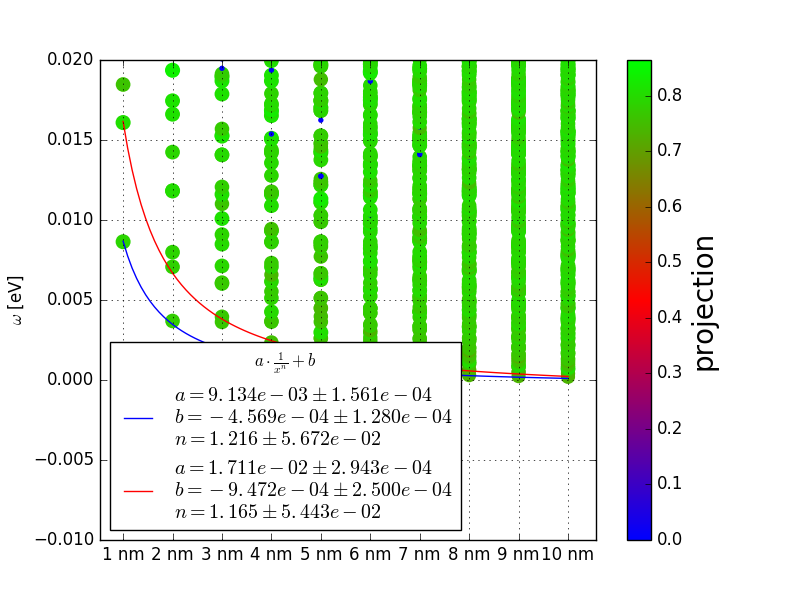
\includegraphics[width=\columnwidth]{Figures/FrequencyModeProjectionsZoomFit.eps}
    \caption{Frequency plotted as a function of hole size. Every green dot being a specific mod, and the red and blue lines being trend curves for the first and second mod.}
    \label{size vs frequency}
\end{figure}
\twocolumngrid
Looking at the data it is clear to see that the frequency decreases when the size of the hole increase. Using the regression for the first and second mode it is determined that the relation between frequency and hole size can be described by:
\begin{equation}
    f=a\cdot\dfrac{1}{x^n}
\end{equation}
Where $f$ is the frequency, $x$ is the size of the holes, and where $a$ and $n$ are constant. Compering the constants for the first mode to the constants for the second it is seen that $a$ decreases while $n$ increases. This changes in constants all lead to a more rapid decrease in frequency the higher the mode which is looked at is. This trend can also be used as a scaling factor to predict the frequency for even bigger holes, for example: If you want a 20 nm hole we can predict that the frequency of first mode for this hole will be
\begin{eqnarray*}
    f=\left(8.743\cdot10^{-3}\pm2.012\cdot10^{-4}\right)\cdot\dfrac{1}{20^{1.428\pm5.166\cdot10^{-2}}}\\=1.213\cdot10^{-4}\pm 1.898\cdot 10^{-5} \mathrm{eV}
\end{eqnarray*}

\subsubsection{Interlayer interaction}
\onecolumngrid

\begin{figure}[H]
    \centering
    \includegraphics[width=\columnwidth]{Figures/FrequencyModeProjectionsZeta.eps}
    \caption{$\epsilon=0.31$, $\epsilon=1.00$, $\epsilon=10.0$}
    \label{}
\end{figure}
\twocolumngrid